% compile with XeLaTeX or LuaLaTeX
\documentclass[10pt,a5paper,twoside]{article}
\usepackage[top=12mm,bottom=26mm,outer=28mm,inner=14mm,foot=14mm]{geometry}
\usepackage{calc}
\usepackage{scrextend}
\deffootnote[1.5em]{0em}{1em}{\thefootnotemark\quad}
\renewcommand{\footnoterule}{%
  \kern -2.4pt
  \hrule width \textwidth height 0.4pt
  \kern 2pt
}

\usepackage{fontspec}
\setmainfont[
	Ligatures=TeX,
	Extension=.otf,
	SlantedFont=cmunsl,
	BoldFont=cmunbx,
	ItalicFont=cmunti,
	BoldItalicFont=cmunbi,
	SmallCapsFont=cmunrm, % for upright instead of slanted small caps
	SmallCapsFeatures={Letters=SmallCaps},	
]{cmunrm}

\usepackage{microtype,ellipsis}

\usepackage{polyglossia}
\setotherlanguage{russian} % the name of the original Russian version at the end of this book is written using Cyrillic letters

\usepackage{textcomp}

\usepackage{amsmath,amssymb,nicefrac,amscd}
\usepackage{graphicx,float}
\usepackage{pdfpages}

\usepackage{enumitem}
\setitemize[1]{noitemsep,nosep,leftmargin=0.99em,label={--}}

\usepackage{transparent}
\usepackage{csquotes}
\usepackage{siunitx}
\sisetup{per-mode=fraction,fraction-function=\nicefrac}
\DeclareSIUnit[number-unit-product=\,]\uhr{Uhr}
\DeclareSIUnit[number-unit-product=\,]\zoll{Zoll}

\usepackage{hyperref}

\usepackage{todonotes}

\newcommand{\eps}{\varepsilon}
\newenvironment{problem}[1]{\paragraph*{#1}}{}
\newenvironment{note}[1]{\par\noindent\textsc{#1} }{\par}

\setdefaultlanguage{turkish}

\title{5'inden 15'ine çocuklar için problemler}

\author{V.\,I.~Arnold
\vspace*{2cm}\\
\includegraphics[width=\linewidth]{resources/photo-arnold_small}
}
\date{}

\newcommand\ba{\begin{array}}
\newcommand\ea{\end{array}}
\newcommand{\ra}{\rightarrow}

\begin{document}
\maketitle
\thispagestyle{empty}
\cleardoublepage
\setcounter{page}{1}
\begin{abstract}

Bu kitapçık, düşünme kültürünün gelişmesi için yazar ta\-ra\-fın\-dan seçilmiş ya da tasarlanmış 77 problemden oluşmaktadır. Bu prob\-lem\-lerin çoğu, genel eğitim dışında herhangi özel bir bilgi gerektirmemektedir. Yine de, problemlerden bazıları üniversite profesörleri için bile zorlayıcı olabilir.

Kitapçık ilkokuldan  üniversiteye kadar tüm düzeyde  öğren\-ci\-le\-re, öğretmenlere, anne-babalara -- ve düşünme kültürünü kişisel gelişimin  asli bir parçası olarak gören herkese -- sunulmuştur.
\end{abstract}
\clearpage

\section*{Preface}
2004 baharında Paris'te, Rus Parisliler küçük çocuklarına Rusya'da bir gelenek olan  düşünme kültürünü kazandırmak için benden yardım istediklerinde bu problemleri kağıda döktüm.

Bu kültürün, her şeyden önce basit olan ama kolay olmayan sorular üstüne  erken ve  bağımsız düşünmeyle  ekildiğine derinden kaniyim. (1., 3. ve 13. problemleri hararetle öneririm.)

Uzun yılların deneyimi, okulda geri kalan {\em alıkların} bu problemleri 10~numara öğrencilerden çoğunlukla daha iyi çözdüklerini söylüyor bana; 
çünkü o öğrencilerin  --sınıfın en gerisinde hayatta kalabilmek ve--
Figaro'nun kendisi için dediği gibi  \enquote{tüm  Seville ve  Granada'yı yönetmek için},
kesintisiz biçimde gereğinden daha fazla düşünmeleri gerekiyor. Öte yandan 10~numara öğrenciler  bu problemlerde \enquote{neyin neyle çarpılacağını} bir türlü yakalayamıyor. 

Ayrıca, beş yaşındaki çocukların benzer problemleri eğitim ile bo\-zul\-muş öğrencilerden daha iyi 
çözdüklerini de fark ettim; ama bu öğrenciler de, bu problemlerle, ineklemeye alışmış üniversite öğ\-ren\-ci\-le\-rin\-den daha iyi başa çıkıyor; yine de bu üniversite öğrencileri pro\-fe\-sör\-le\-ri\-ni alt ediyor (bu basit problemleri çözmede en kötüler Nobel ve Fields ödülü sahipleri).

\clearpage
\section*{Problemler}


%\usepackage[mathcal]{euscript}
%\usepackage{mathrsfs}
%\usepackage{amsfonts,amssymb,amsbsy,amsmath}
%\usepackage{graphicx,color}
%\usepackage{epsfig}
%\usepackage[utf8]{inputenc}
%\usepackage[turkish]{babel}
%\usepackage{verbatim}



 
\begin{problem}{1.}
	İlk okuma kitabını alabilmek için Nuriye'nin 7 kuruşa daha ihtiyacı varmış, Nuri'nin  ise 1 kuruşa daha ihtiyacı varmış. Ortaklaşa bir kitap alıp birlikte kullanmak için paralarını birleştirmişler ama böyle bile paraları yetmemiş. Kitap kaç kuruşmuş?
\end{problem}

\begin{problem}{2.}
	Mantarıyla birlikte bir şişe 10 kuruş ediyor. Sadece şişenin fiyatı mantarınkinden 9 kuruş fazla. Mantarsız bir şişe kaç kuruş eder?
\end{problem}


\begin{problem}{3.}
Bir tuğlanın ağırlığı, yarım tuğla ve 1 kilonun ağırlığı kadar. Bir tuğla kaç kilo?
\end{problem}

\begin{problem}{4.}
Bir fıçı şaraptan bir kaşık şarap alıp  (tam dolu olmayan) bir bardak çaya dökülüyor. Ardından, bardaktaki (homojen olmayan) ka\-rı\-şım\-dan aynı kaşıkla bir kaşık alınıp varile geri dökülüyor. Böylece hem varilde hem bardakta diğer taraftan gelmiş bir miktar sıvı bu\-lu\-nu\-yor (varilde çay, bardakta şarap). Hangisinde diğer taraftan gelmiş sıvının hacmi daha fazladır: bardakta mı, varilde mi?
\end{problem}

\begin{problem}{5.}
İki yaşlı kadın, şafak sökerken $A$'dan $B$'ye ve $B$'den $A$'ya bir\-bir\-le\-ri\-ne doğru yola çıkmışlar. Tam öğle vakti karşılaşmışlar ama hiç durmadan, aynı hızda yürümeye devam etmişler. Birinci kadın ($B$'ye) akşamüstü 4'te varmış; ikinci kadınsa ($A$'ya) akşam 9'da varmış. O gün şafak kaçta sökmüş?
\end{problem}

\begin{problem}{6.}
(Standart bir Amerikan sınavında) Dik bir üçgenin hipotenüsü \SI{10}{\cm}.dir; üstüne düşen yükseklik ise \SI{6}{\cm}~cm.dir. Üçgenin alanı ne kadardır?

Amerikalı öğrenciler bu problemle onlarca yıldır  rahatlıkla baş ediyordu. Sonra Moskova'dan öğrenciler gelmeye başladı ve (cevap olarak 30~santimetre~kare veren) Amerikalı arkadaşlarının çözebildiği bu soruyu çözemediler. Niye?
\end{problem}

\begin{problem}{7.}
Vahit'in kızkardeşlerinin sayısı erkek kardeşlerinden iki fazla. Va\-hit'\-in anne ve babasının kızlarının sayısı oğullarının sayısından kaç fazla?
\end{problem}

\begin{problem}{8.}
Güney Amerika'da yuvarlak bir göl vardır. Her yıl 1~Haziran'da bir Victoria Regia çiçeği tam merkezde belirir (gövdesi dipten yükselir ve taç yaprakları tıpkı nülüfer gibi suyun üstüne yayılır). Her gün çiçeğin alanı iki katına çıkar, ve 1~Temmuz'da tüm gölü kaplamış olur, taç yapraklarını döker ve tohumları dibe batar. Hangi gün, çiçeğin alanı gölün alanının yarısı kadardır?
\end{problem}

\begin{problem}{9.}
Bir köylü bir kurt, bir keçi ve bir lahanayı bir tekneyle nehrin karşısına götürmek zorundadır. Tekne o kadar küçüktür ki her defasında
bu üçünden ancak birini  teknede yanına alabilmektedir.   Bu üçünü de karşıya nasıl taşıyacak? (Kurt keçiyle yalnız bırakılamaz, keçi de lahanayla yalnız bırakılamaz.)
\end{problem}

\begin{problem}{10.}
Gün boyunca bir direğe \SI{3}{\cm} tırmanan bir salyangoz, gece bo\-yun\-ca uyuyakaldığından istemeden \SI{2}{\cm} aşağıya kaymaktadır. Direğin u\-zun\-lu\-ğu \SI{10}{\metre}.dir ve tam tepesinde (elbette salyangoz için) leziz bir şeker bu\-lun\-mak\-ta\-dır. Salyangoz kaç günde şekeri alabilecektir?
\end{problem}

\begin{problem}{11.}
Bir kampçı çadırından \SI{10}{\km} güneye yürümüş, doğuya dönmüş, tam doğu yönünde \SI{10}{\km} daha yürümüş, kuzeye dönmüş ve \SI{10}{\km} daha yürüyünce kendini çadırının yanında bulmuş. Ayının rengi neymiş ve tüm bunlar nerede olmuş?
\end{problem}

\begin{problem}{12.}
Denizin gelgiti bugün öğlen 12'de en yukarıdaydı. Yarın aynı yerde kaçta yukarıda olacak?
\end{problem}

\begin{problem}{13.}
Puşkin'in iki cildi, birinci ve ikinci cildi, bir rafta sırt sırta duruyor. Her bir cildin sayfaları toplam \SI{2}{\cm} kalınlığında, ve ön ve arka kapağın her biri \SI{2}{\mm} kalınlığında. Bir kitap kurdu (sayfalara dik bir biçimde) kemirerek 1.~cildin birinci sayfasından 2.~cildin son sayfasına yolunu açmış. Kitap kurdunun yolunun uzunluğu kaç cm.dir? [İnanılmaz bir cevabı olan (4~mm) bu topoloji problemi akademikler için imkansızdır, ama okulöncesi kimi çocuklar bu soruyu kolayca halleder.]
\end{problem}

\begin{problem}{14.}
Yukarıdan ve önden görünüşü aşağıda  (politop olarak) resmedilen  cismi bulun. Yandan görünüşünü çizin (politopun görünmeyen ke\-nar\-la\-rı\-nı kesikli çizgiyle göstererek).
	\begin{figure}
		\footnotesize
		\null\hfill
		\parbox{0.2\linewidth}{\centering\includegraphics{resources/taskbook-99}\\ Yukarıdan görünüş}
		\hfill
		\parbox{0.2\linewidth}{\centering\includegraphics{resources/taskbook-98}\\ Önden görünüş}
		\hfill\null
	\end{figure}
\end{problem}

\begin{problem}{15.}
64 sayısı 10 tane doğal sayının (1'den büyükeşit tamsayılar) toplamı olarak kaç yolla yazılabilir? [Terimlerinin sadece sıraları de\-ğiş\-miş  toplama yolları birbirinden farklı sayılmaz.]
\end{problem}

\begin{problem}{16.}
Birkaç çubuğu (örneğin domino taşlarını) üstüste koyarak $x$ u\-zun\-lu\-ğun\-da bir parça dışarı taşırılabilir.  Bu $x$ dışarı taşma uzunluğunun elde e\-di\-le\-bi\-le\-cek en büyük değeri  nedir?
	\begin{figure}
		\includegraphics{resources/taskbook-97}
	\end{figure}
\end{problem}

\begin{problem}{17.}
$A$ ve $B$ şehirleri arasındaki uzaklık \SI{40}{\km}.dir. İki bisikletli aynı anda $A$ ve $B$ şehirlerinden birbirlerine doğru yola çıkarlar; birinin hızı \SI{10}{\km\per\hour} diğerinin \SI{15}{\km\per\hour}'dir. Bir sinek \SI{100}{\km\per\hour} hızla, ilk bisikletçiyle birlikte $A$ şehrinden uçmaya başlar, ikinci bisikletçiye ulaşır, alnına dokunur, birinciye geri uçar, onun alnına dokunur, ikinciye geri döner ve böyle, bisikletçilerin alınları birbirine çarpıp da arada ezilinceye kadar devam eder. Sinek toplam kaç km. uçmuştur?
	\begin{figure}
		\includegraphics{resources/taskbook-1}
	\end{figure}
\end{problem}

\begin{problem}{18.}
Bir domino taşı satranç tahtasının iki karesini kaplar.  (Aynı köşegende) karşılıklı iki kare dışında tahtanın tüm karelerini 31 adet domino taşıyla kaplayın. [Bir satranç tahtasında $8 \times 8 = 64$ kare vardır.]
	\begin{figure}
		\includegraphics{resources/taskbook-2}
	\end{figure}
\end{problem}

\begin{problem}{19.}
Bir kırkayak küp şeklinde bir odanın bir köşesinden (tabanda soldaki köşeden) karşı köşeye (tavanda sağdaki köşeye) sürünmek istiyor. Odanın duvarları üzerinde böyle bir yolculuk için en kısa yolu bulun.
	\begin{figure}
		\includegraphics{resources/taskbook-3}
	\end{figure}
\end{problem}

\begin{problem}{20.}
5 ve 3~litrelik iki kabınız var. (Kapların birinde olacak biçimde) 1~litre elde edin.
	\begin{figure}
		\includegraphics{resources/taskbook-4}
	\end{figure}
\end{problem}


\begin{problem}{21.}
Bir ailede 5 kafa ve 14 bacak vardır. Bu ailede kaç insan ve kaç köpek vardır?
\end{problem}

\begin{problem}{22.}
	Bir $ABC$ üçgeninin üç kenarı $AB$, $AC$ ve $BC$ üzerinde dışa doğru eşkenar üçgenler çiziliyor. Merkezlerinin ($*$) bir eşkenar üçgen oluşturduğunu kanıtlayın.
	\begin{figure}
		\includegraphics{resources/taskbook-6}
	\end{figure}
\end{problem}

\begin{problem}{23.}
	Bir kübün bir düzlemle arakesitiyle hangi çokgenler elde edilir? Bir beşgen elde edebilir miyiz? Yedigen? Düzgün altıgen?
	\begin{figure}
		\includegraphics{resources/taskbook-7}
	\end{figure}
\end{problem}

\begin{problem}{24.}
	Bir kübün merkezinden geçen öyle bir doğru çizin ki kübün sekiz köşesinin bu doğruya uzaklıklarınn kareleri toplamı (benzer tüm doğrulara kıyasla) a) en fazla, b) en az olsun.
\end{problem}

\begin{problem}{25.}
	Dik çembersel bir koni, bir düzlem ile kapalı bir eğri boyunca kesiliyor. Koninin içine sıkıştırılmış iki küre, biri $A$ diğeri $B$ noktasında olmak üzere, bu düzleme teğet olsun. Arakesit eğrisinde öyle bir $C$ noktası bulun ki $CA + CB$ uzaklıklar toplamı olası a) en fazla, b) en az olsun.
	\begin{figure}
		\includegraphics{resources/taskbook-9}
	\end{figure}
\end{problem}

\begin{problem}{26.}
	Dünya yüzeyinden, meridyenlere ekvator noktalarında çizilen teğet doğruların oluşturduğu silindire, ekvatora paralel olan ve dün\-ya\-nın kutuplar ekseninden geçen ışınlar boyunca izdüşüm alınıyor. Fran\-sa'nın izdüşümünün alanı Fransa'nın kendi alanından büyük mü küçük mü olacaktır?
	\begin{figure}
		\includegraphics{resources/taskbook-10}
	\end{figure}
\end{problem}

\begin{problem}{27.}
	$p$ tek asal olmak üzere $2^{p-1}$ sayısının $p$'ye bölümünden kalanın 1 olacağını kanıtlayın (Örnekler: $2^2 = 3a + 1$, $2^4 = 5b+1$, $2^6 = 7c+1$, $2^{10} - 1 = 1023 = 11\cdot 93$.)
\end{problem}

\begin{problem}{28.}
	\SI{10}{\cm} uzunluğunda bir iğne, çizgi aralığı da \SI{10}{\cm} olan bir çizgili kağıt üzerine rastgele atılıyor. Bu $N$ (bir milyon) kez tekrarlanıyor. Atılan iğneler kaç kez (yaklaşık olarak, yüzde birkaç hata ile) kağıttaki herhangi bir çizgiyi kesecektir?
	\begin{figure}
		\includegraphics{resources/taskbook-12}
	\end{figure}
Bu deney, bir milyon atışla olmasa da (benim de 10 yaşında yap\-tı\-ğım gibi) $N=100$ için yapılabilir. [Bu problemin cevabı şaşırtıcı: $\frac{2}{\pi}N$. Üstelik, uzunluğu $a \cdot \SI{10}{\cm}$ olan eğilmiş bir iğne için bile $N$ atışta gözlenen kesişim sayısı yaklaşık olarak $\frac{2a}{\pi}N$ olacaktır. $\pi$ sayısı $\approx \frac{355}{113}\approx \frac{22}{7}$.]
\end{problem}

\begin{problem}{29.}
	Üçgen yüzleri olan çokyüzlüler, örneğin şu Platon cisimleridir: dörtyüzlü (4~adet yüz), sekizyüzlü (oktahedron, 8~adet), yirmiyüzlü (ikosahedron, 20 adet -- tüm yüzler aynı; bunu çizmek ilginç olacaktır, 12~köşesi ve 30~kenarı var.)
	\begin{figure}
		\footnotesize
		\null\hfill
		\parbox{0.3\linewidth}{\centering\includegraphics{resources/taskbook-131}\\Dörtyüzlü (tetrahedron, $\text{tetra}= 4$)}
		\hfill
		\parbox{0.3\linewidth}{\centering\includegraphics{resources/taskbook-132}\\Sekizyüzlü (oktahedron ($\text{octo}= 8$)}
		\hfill\null\\
		{\Huge ?}\\Yirmiyüzlü
	\end{figure}
Böyle çokyüzlüler (sınırlı, dışbükey, üçgen yüzlü) için yüz sayısının, köşe sayısının 2 katından 4 eksik olduğu doğru mudur?

Bir başka Platon cismi (toplam 5 tane var):
	\begin{figure}
		\includegraphics{resources/taskbook-14}
	\end{figure}
\end{problem}

\begin{problem}{30.}
	Onikiyüzlü, 12~adet (düzgün) beşgen yüzü, 20~köşesi ve 30~kenarı olan dışbükey bir çokyüzlüdür (köşeleri, bir yirmiyüzlünün yüzlerinin merkezleridir).

Bir onikiyüzlünün içine kenarları onikiyüzlünün yüzlerinin kö\-şe\-gen\-leri olacak (ve her bir kübün köşeleri onikiyüzlünün köşeleri olacak) biçimde 5~adet küp koyun (Bir kübün, onikiyüzlünün her yüzüne bir tane olmak üzere, 12~kenarı vardır). [Kepler bunu gezegenler için icat etmiştir.]
\end{problem}

\begin{problem}{31.}
	Bir kübün içine (köşeleri kübün köşeleri ve kenarları kübün yüz\-le\-ri\-nin köşegenleri olacak biçimde) konmuş iki dörtyüzlünün kesişimini bulun.
Kübün hacminin kaçta kaçı bu kesişimin içinde yer alır?
\end{problem}


\begin{problem}{31\textsuperscript{tekrar}.}
Bir kübün kenarlarında verilen üç noktadan geçen düzlemin küple arakesitini inşa edin. [Düzlemsel arakesitin kübün yüzlerini kes\-ti\-ği çokgeni çizin.]
	\begin{figure}
		\includegraphics{resources/taskbook-15}
	\end{figure}
\end{problem}


\begin{problem}{32.}
Bir dörtyüzlünün kaç simetrisi vardır? Bir kübün? sekizyüzlünün? yirmiyüzlünün? onikiyüzlünün? Simetri, uzunlukları koruyan bir dö\-nü\-şüm\-dür.
Bunlardan kaç tanesi döndürme, kaç tanesi yansımadır (sıralanan beş durumun her biri için)? 
\end{problem}

\begin{problem}{33.}
Özdeş küplerin $6$ yüzünü, $6$ renk ($1,\dotsc,6$) kullanarak her yüze bir renk boyamanın kaç yolu vardır öyle ki boyanmış herhangi iki küp aynı olmasın (yani biri diğerinden bir döndürme ile elde edilemesin)?
	\begin{figure}
		\includegraphics{resources/taskbook-17}
	\end{figure}
\end{problem}

\begin{problem}{34.}
$n$ adet nesneyi sıralamanın kaç değişik yolu vardır?
$n=3$ için altı yol var: $(1,2,3)$, $(1,3,2)$, $(2,1,3)$, $(2,3,1)$, $(3,1,2)$, $(3,2,1)$. Peki nesnelerin sayısı $n=4$ olursa? $n=5$? $n=6$? $n=10$?  
	\begin{figure}
		\includegraphics{resources/taskbook-18}
	\end{figure}
\end{problem}

\begin{problem}{35.}
	Bir kübün $4$ uzun köşegeni vardır. Bu dört köşegenin kaç farklı permütasyonu kübün döndürmeleriyle elde edilir?
	\begin{figure}
		\includegraphics{resources/taskbook-19}
	\end{figure}
\end{problem}

\begin{problem}{36.}
	Üç tamsayının küplerinin toplamı, bu sayıların toplamının kü\-bün\-den çıkarılıyor. Fark her zaman $3$'e bölünebilir mi?
\end{problem}

\begin{problem}{37.}
	$5$. kuvvetler ve $5$'e bölünebilirlik için, ve $7$. kuvvetler ve $7$'ye bölünebilirlik için aynı soru.\end{problem}

\begin{problem}{38.}
Şu toplamı hesaplayın:
	\begin{equation*}
		\frac{1}{1\cdot 2} + \frac{1}{2\cdot 3} + \frac{1}{3\cdot 4} + \dotsb + \frac{1}{99\cdot 100}
	\end{equation*}
(cevabın $\%1$'ini geçmeyecek bir hata ile).
\end{problem}

\begin{problem}{39.}
	İki çokgen eşit alanlara sahipse, sonlu sayıda çokgensel parçaya öyle ayrılabilirler ki bu parçaları tekrar bir araya getirerek hem birinci hem de ikinci çokgen elde edilebilir. İspatlayın! 
[Uzaysal cisimler için bu doğru değildir: aynı hacme sahip bir küp ve bir dörtyüzlü bu şekilde parçalanamazlar!] 
	\begin{figure}
		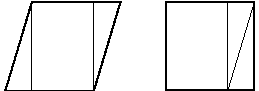
\includegraphics{resources/q39_horizontal}
	\end{figure}
\end{problem}

\begin{problem}{40.}
	Bir paralelkenarın dört köşesi, bir parça kareli kağıdın kare kö\-şe\-le\-rin\-de seçilmiş. Paralelkenarın kenarlarında da içinde de kareli  kağıdın başka bir kare köşesi olmadığı görülmüş.
Böyle bir paralelkenarın ala\-nı\-nın kağıdın bir karesinin alanına eşit olduğunu ispatlayın.
	\begin{figure}
		\includegraphics{resources/taskbook-24}
	\end{figure}
\end{problem}

\begin{problem}{41.}
	40. sorudaki koşullar altında, paralelkenarın içinde $a$ tane, ke\-nar\-la\-rın\-da $b$ tane kare köşesi  olduğu görülmüş. Paralelkenarın alanını hesaplayın.
\end{problem}

\begin{problem}{42.}
40. sorudaki önerme, 3~boyutlu uzayda paralelçokyüzlü için doğru mudur?
\end{problem}

\begin{problem}{43.}
	Tavşan (ya da Fibonacci) sayıları $1,2,3,5,8,\allowbreak 13,21,34,\dotsc$ dizisini oluşturur; burada herhangi bir $n=1,2,\dotsc$ için $a_{n+2}=a_{n+1}+a_{n}$'dir ($a_n$ dizideki $n$. sayıdır). $a_{100}$ ve $a_{99}$ sayılarının en büyük ortak bölenini bulun.
\end{problem}

\begin{problem}{44.}
	Dışbükey bir $n$-geni kesişmeyen köşegenlerinden üçgenlere ayırma yollarının (Katalan) sayısını bulun. Örneğin, $c(4)=2$, $c(5)=5$, $c(6)=14$. Peki $c(10)$ nasıl bulunur?
	\begin{figure}
		\includegraphics{resources/taskbook-281}
		\qquad
		\includegraphics{resources/taskbook-282}
	\end{figure}
\end{problem}

\begin{problem}{45.}
	Bir kupa turnuvasına $n$ takım katılıyor, kaybeden takım tur\-nu\-va\-dan ayrılıyor ve kupa galibi $n-1$ oyun sonunda belli oluyor. 
	Turnuva fikstürü sembollerle  yazılabilir: örneğin $((a,(b,c)),d)$,  "$b$ ile $c$ oynar, galip $a$ ile karşılaşır, bunların galibi $d$ ile karşılaşır" demek oluyor.
	10 takım için farklı fikstürlerin sayısı kaçtır?
	\begin{itemize}
		\item 2 takım için sadece $(a,b)$ var ve sayısı 1.
		\item 3 takım için sadece $((a,b),c)$, or $((a,c),b)$, or $((b,c),a)$ var ve sayısı 3.
		\item 4 takım için:
			\begin{equation*}
				\begin{array}{@{}cccc@{}}
					(((a,b),c),d) & \quad\;(((a,c),b),d) & \quad\;(((a,d),b),c) & \quad\;(((b,c),a),d) \\
					(((b,d),a),c) & \quad\;(((c,d),a),b) & \quad\;(((a,b),d),c) & \quad\;(((a,c),d),b) \\
					(((a,d),c),b) & \quad\;(((b,c),d),a) & \quad\;(((b,d),c),a) & \quad\;(((c,d),b),a) \\
					((a,b),(c,d)) & \quad\;((a,c),(b,d)) & \quad\;((a,d),(b,c))
				\end{array}
			\end{equation*}
	\end{itemize}
\end{problem}

\begin{problem}{46.}
	$n$ adet noktayı ($1, 2, \dotsc, n$ olsunlar), bir ağaç oluşturacak şekilde ($n-1$ adet) doğru parçasıyla birleştirin. Kaç farklı ağaç elde edilebilir? (Daha $n=5$ durumu bile ilginç!)

	$n=2$:\quad \includegraphics{resources/taskbook-291}\,,\quad sayısı 1;

	$n=3$:\quad
	\includegraphics{resources/taskbook-292}\,,\quad
	\includegraphics{resources/taskbook-293}\,,\quad
	\includegraphics{resources/taskbook-294}\,,\quad
	sayısı 3;

	$n=4$:\quad\def\quad{\hskip.7em}
	$\vcenter{\hbox{\includegraphics{resources/taskbook-295}}}$,\quad
	$\vcenter{\hbox{\includegraphics{resources/taskbook-296}}}$,\quad
	$\vcenter{\hbox{\includegraphics{resources/taskbook-297}}}$,\quad
	$\vcenter{\hbox{\includegraphics{resources/taskbook-298}}}$,\quad
	$\vcenter{\hbox{\includegraphics{resources/taskbook-299}}\hbox{\includegraphics{resources/taskbook-290}}
	\vskip-8pt
	\hbox to50bp{\dotfill}}$,\\
	\null\hspace{\parindent}\phantom{$n=4$:}\quad sayısı 16.
\end{problem}

\begin{problem}{47.}
$\{1,2,\ldots,n\}$ sayılarının bir $(x_1,\ldots,x_n)$ permütasyonuna, eğer $x_1<x_2>x_3<x_4\ldots$ koşulunu sağlıyorsa, ($n$ uzunluğunda) bir {\it yılan} denir.

	\begin{note}{ÖRNEK:}
		\begin{equation*}
			\begin{aligned}[t]
				&\begin{aligned}[t] n=2, \text{\ \ sadece \ \ } 1<2, \end{aligned} &&\text{sayısı }1, \\
				&\hskip-\nulldelimiterspace\mathord{\left.\begin{aligned} n=3, \hphantom{\text{\ \ only\ \ }} 1&<3>2 \\
				2&<3>1\end{aligned} \right\}}, && \text{sayısı }2, \\
				&\hskip-\nulldelimiterspace\mathord{\left.\begin{aligned} n=4, \hphantom{\text{\ \ only\ \ }} 1&<3>2<4 \\
				1&<4>2<3 \\
				2&<3>1<4 \\
				2&<4>1<3 \\
				3&<4>1<2\end{aligned} \right\}},
				&&\text{sayısı }5. \\
			\end{aligned}
		\end{equation*}
	\end{note}
	$10$ uzunluğunda yılanların sayısını bulun.
\end{problem}

\begin{problem}{48.}
	$n$ uzunluğundaki yılanların sayısı $s_n$ olsun:
	\begin{equation*}
		s_1=1, \quad s_2=1, \quad s_3=2, \quad s_4=5, \quad s_5=16, \quad s_6=61.
	\end{equation*}
	Tanjant fonksiyonunun Taylor serisinin
	\begin{equation*}
		\tan x=1\, \frac{x^1}{1!}+2\, \frac{x^3}{3!}+16\, \frac{x^5}{5!}+\dots=
		\textstyle\sum\limits_{k=1}^{\infty} s_{2k-1}\, \frac{x^{2k-1}}{(2k-1)!}.
	\end{equation*}
olduğunu ispatlayın.
\end{problem}

\begin{problem}{49.}
	Şu serinin toplamını bulun:
	\begin{equation*}
		1+1\, \frac{x^2}{2!}+5\, \frac{x^4}{4!}+61\, \frac{x^6}{6!}+\dots=
		\textstyle\sum\limits_{k=0}^{\infty} s_{2k}\,\frac{x^{2k}}{(2k)!}.
	\end{equation*}
\end{problem}

\begin{problem}{50.}
	$s>1$ için, 
	\begin{equation*}
		\textstyle\prod\limits_{p=2}^{\infty} \frac{1}{1-\frac{1}{p^s}}=\textstyle\sum\limits_{n=1}^{\infty} \frac{1}{n^s}.
	\end{equation*}
özdeşliğini gösterin. (Çarpım tüm $p$ asal sayıları üzerinden, toplam ise tüm $n$ doğal sayıları üzerinden.)
\end{problem}

\begin{problem}{51.}
	Şu serinin toplamını bulun:
	\begin{equation*}
		1+ \frac{1}{4}+ \frac{1}{9}+\dots=\textstyle\sum\limits_{n=1}^{\infty} \frac{1}{n^2}.
	\end{equation*}
	[Toplamın $\nicefrac{\pi^2}{6}$ olduğunu, yani yaklaşık $\nicefrac{3}{2}$ olduğunu kanıtlayın.]
\end{problem}

\begin{problem}{52.}
	Bir  $\nicefrac{p}{q}$ kesrinin basit olma olasılığını bulun  (bu olasılık şöyle tanımlanıyor:
	$p^2+q^2 \leqslant R^2$ dairesinde, $p$ ve $q$'nun 1'den büyük ortak böleni olmayacak biçimde $(p,q)$ vektörlerinin sayısını ($N(R)$) bu\-lu\-yo\-ruz, bunun ardından basit kesir olma olasılığı 
$\nicefrac{N(R)}{M(R)}$ oranının limiti oluyor. Burada  $M(R)$ dairedeki tamsayı noktaların sayısı $(M \sim \pi R^2)$).
	\begin{figure}
		\includegraphics{resources/taskbook-36}\\
		\footnotesize $M(5)=81$, $N(5)=44$, $\nicefrac{N}{M} = \nicefrac{44}{81}$
	\end{figure}
\end{problem}

\begin{problem}{53.}
Problem~43'teki  $a_n$ Fibonacci sayı dizisi için, $n$ sonsuza giderken
	$a_{n+1}/a_n$ oranının limitini bulun:\vspace{2\jot}
	\begin{equation*}
		\frac{a_{n+1}}{a_n}=2,\ \frac 32,\ \frac53, \ \frac85, \ \frac{13}8,
		\ \frac{34}{21}.
	\end{equation*}
	[Cevap \enquote{altın oran},
	$\frac{\sqrt{5}+1}{2\vphantom)} \approx 1.618$. Bu oran, bir karttan kısa kenarı uzunlukta kenarları olan bir karenin kesip çıkarılmasından sonra kalan kısmın karta  benzer olması durumunda  kartın kenarlarının oranına eşittir, yani resimde
	$\frac{AB}{BC}=\frac{PC}{CD}$. Altın oran, düzgün beşgenle ve beş kollu yıldızla nasıl ilişkilidir?]
	\begin{figure}
		\includegraphics{resources/taskbook-37}
	\end{figure}
\end{problem}

\begin{problem}{54.}
	$a_{2k}=1$ ve $a_{2k+1}=2$ olmak üzere şu sonsuz süregiden kesri hesaplayın:
	\begin{equation*}
		1+\cfrac{1}{2+\cfrac{1}{1+\cfrac{1}{2+\cfrac{1}{1+\cfrac{1}{2+\ldots}}}}}=
		a_0+\cfrac{1}{a_1+\cfrac{1}{a_2+\cfrac{1}{a_3+\dots}}}
	\end{equation*}
	 (yani, $n \to \infty$ için
	\begin{equation*}
		a_0+\cfrac{1}{a_1+\cfrac{1}{a_2+{\atop{\ddots \atop {}} + \cfrac{1}{a_n}}}}
	\end{equation*}
	kesirlerinin limitini bulun).
\end{problem}

\begin{problem}{55.}
	$|x| \leqslant 1$ olmak üzere 
	\begin{equation*}
		y=\cos 3 (\arccos x),\ y=\cos 4 (\arccos x),\
		y=\cos n (\arccos x)
	\end{equation*}
	polinomlarını bulun.
\end{problem}

\begin{problem}{56.}
	1'in $n$ tane $n$-inci kompleks kökünün $k$-inci üslerinin  toplamını bulun.
\end{problem}

\begin{problem}{57.}
	$(x,y)$-düzleminde, parametrik olarak
	\begin{equation*}
		\{x=\cos 2t, y=\sin 3t\},\quad
		\{x=t^3-3t, y=t^4-2t^2\}
	\end{equation*}
diye verilen eğrileri çizin.
\end{problem}

\begin{problem}{58.}
	$\int_0^{2\pi} \sin^{100} x\,dx$  integralini hesaplayın (cevabın \%10'unu geç\-me\-ye\-cek bir hata ile).
\end{problem}

\begin{problem}{59.}
	$\int_1^{10} x^x\,dx$ integralini hesaplayın (cevabın \%10'unu geçmeyecek bir hata ile).
\end{problem}

\begin{problem}{60.}
	Yarıçapı 1 olan bir küre üzerinde iç açıları $(\alpha, \beta, \gamma)$ olan ve 
	kenarları büyük çemberler (kürenin merkezinden geçen düzlemlerin küreyle arakesitleri) olan bir üçgenin alanını hesaplayın.

	\begin{note}{CEVAP:}
		$S=\alpha+\beta+\gamma-\pi$ (örneğin, üç açısı da dik açı olan bir üçgen için, $S=\nicefrac{\pi}{2}$, yani kürenin toplam alanının 8'de 1'i).
		\begin{figure}
			\null\hfill
			\includegraphics{resources/taskbook-44}
			\hfill
			\includegraphics{resources/taskbook-45}
			\hfill\null
		\end{figure}
	\end{note}
\end{problem}

\begin{problem}{61.}
	Yarıçapı $r$ olan bir çember, yarıçapı 1 olan bir çemberin içinde (kaymadan) yuvarlanıyor.
	Yuvarlanan çemberin bir noktasının tüm izini $r=\nicefrac{1}{3}$,  $r=\nicefrac{1}{4}$, $r=\nicefrac{1}{n}$ ve $r=\nicefrac{1}{2}$ için çizin (bu ize hiposikloit denir).
\end{problem}

\begin{problem}{62.}
	$n$ öğrencili  bir sınıfta,  aynı yaşgününe sahip iki öğrenci olma olasılığını tahmin edin. Olasılık yüksek mi düşük mü?

	\begin{note}{CEVAP:}
		Eğer öğrenci sayısı bir $n_0$'ın (çok) üstündeyse olasılık (çok) yüksek,
		eğer $n_0$'ın (çok) altındaysa olasılık (çok) düşük;  bu $n_0$'ın tam olarak kaç olduğu bulunmalı (olasılığın $p \approx \nicefrac{1}{2}$ olduğu an).
	\end{note}
\end{problem}

\begin{problem}{63.}
	Snell (Snellius) kanunu, katmanlı bir ortamda ışık ışınının kat\-man\-la\-ra dik yön ile yaptığı  $\alpha$ açısının
	\begin{equation*}
		n(y) \sin \alpha=\text{sabit},
	\end{equation*}
	eşitliğini sağladığını söyler. Burada  $n(y)$, $y$ yüksekliğindeki katmanın kırılma indisidir (ışığın boşluktaki hızı 1 olarak alınırsa, $n$ ışığın or\-tam\-da\-ki hızıyla ters orantılıdır; suda $n=\nicefrac{4}{3}$).
	\begin{figure}
		\null\hfill
		\includegraphics{resources/taskbook-47}
		\hfill
		\includegraphics{resources/taskbook-471}
		\hfill\null
	\end{figure}

	$n(y)$ indisinin belirli bir yükseklikte en büyük değerine ulaştığı \enquote{çöl üstünde hava} ortamında ışınların izlediği yolları çizin. (Nesnelerden çıkan ışınların imgelerle nasıl ilişkili olduğunu bilenlere bu problemin çözümü çöldeki serapları açıklayacaktır.) 
\end{problem}

\begin{problem}{64.}
	Tüm  açıları dar olan bir  $ABC$ üçgeninin içine en kısa çevreye sahip  bir  $KLM$ üçgeni oturtun	($K$ köşesi  $AB$'de, $L$ köşesi    $BC$'de, $M$  ise $CA$'da olacak şekilde).
	\begin{figure}
		\includegraphics{resources/taskbook-48}
	\end{figure}

	\begin{note}{{\. I}PUCU:}
		Dar açılı olmayan bir üçgen için cevap, dar açılı üçgen için bulunacak güzel cevaba benzemiyor. 
	\end{note}
\end{problem}

\begin{problem}{65.}
	$\nicefrac{1}{r}$ fonksiyonunun, merkezi $(X,Y,Z)$ noktasında olan $R$ yarıçaplı  küre üzerinde ortalama değerini  bulun. (Burada $r$ orijine uzaklık, yani $r^2=x^2+y^2+z^2$.)

	\begin{note}{{\. I}PUCU:}
		Bu problem Newton'un yerçekimi kanunu ve elektrik ku\-ra\-mın\-da Coulomb kanunu ile ilişkilidir. Problemin iki boyutlu halinde fonksiyon $\ln r$ ve küre yerine çember olacak.
	\end{note}
\end{problem}

\begin{problem}{66.}
	$2^{10}=1024 \approx 10^3$  olması,
	$\log_{10} 2 \approx 0.3$ olmasını gerektirir. Bunların birbirinden ne kadar farklı olduğunu tahmin edin ve $\log_{10} 2$ sayısını virgülden sonra 3. basamağa kadar hesaplayın.
\end{problem}

\begin{problem}{67.}
	Aynı kesinlikle $\log_{10} 4$, $\log_{10} 8$,
	$\log_{10} 5$, $\log_{10} 50$, $\log_{10} 32$, $\log_{10} 128$,
	$\log_{10} 125$, $\log_{10} 64$ değerlerini bulun.
\end{problem}

\begin{problem}{68.}
	$7^2 \approx 50$ olduğunu kullanarak  $\log_{10} 7$ için yaklaşık bir değer bulun.
\end{problem}

\begin{problem}{69.}
	$\log_{10} 64$ ve $\log_{10} 7$ sayılarını kullanarak, $\log_{10} 9$, $\log_{10} 3$,
    $\log_{10} 27$, $\log_{10} 6$, $\log_{10} 12$ değerlerini bulun.
\end{problem}

\begin{problem}{70.}
	$\ln (1+x) \approx x$ eşitliğini kullanarak ($\ln$,  $\log_e$ demek),
\begin{equation*}
		\log_{10} a=\frac{\ln a}{\ln 10}
	\end{equation*}
ilişkisinden\footnote{$e = 2{.}71828\dots$ değerli Euler sayısı, $n\to \infty$ iken
	$\left(1+\frac{1}{n}\right)^n$  dizisinin limiti olarak tanımlanır ve
	$1+\frac{1}{1!} +\frac{1}{2!}+\frac{1}{3!}+\dotsb$ seri toplamına eşittir. Yukarıda 
	 $\ln (1+x)$ için verilen formül ve buradan çıkan $\lim\limits_{x\to 0}\frac{\ln(1+x)}{x} = 1$
eşitliğini kullanarak, $\ln$ altında 1'e giden sayı olarak da tanımlanabilir.}
	%
 ve daha önce hesapladığımız $\log_{10} a$ değerlerinden (ör\-ne\-ğin, $a=128/125, 1024/1000$ vs. için), $\log_{10} e$ ve    $\ln 10$ değerlerini bulun.

	[Şu ana kadar  bulduğumuz sayıların çarpımlarını temel veri olarak kullanarak ve düzeltme için 
	\begin{equation*}
		\ln (1+x) \approx x-\frac{x^2}{2}+\frac{x^3}{3}-\frac{x^4}{4}+\dotsb,
	\end{equation*}
	formülünden yararlanarak, 65.--69. problemlerin çözümleri  yarım sa\-at\-lik bir çalışmayla bize herhangi bir sayının logaritmasının oku\-na\-bi\-le\-ce\-ği dört basamaklı logaritmalar tablosu verir.] (Newton bu yolla 40 basamaklı logaritmalar tablosu oluşturdu!)
\end{problem}

\begin{problem}{71.}
	İkinin üsleri dizisini ele alın: $1$, $2$, $4$, $8$, $16$, $32$, $64$,
	$128$, $256$, $512$, $1024$, $2048, \dotsc$ İlk oniki sayı içinde dört tanesinin ondalık ifadesi 1 ile başlıyor, hiçbiri 7 ile başlamıyor.

	$n \to \infty$ limitinde, $2^m$ sayılarının ($0\leqslant m \leqslant n$) ilk basamaklarının 
	belirli frekanslarla ortaya çıkacağını ispatlayın: \\
	$p_1 \approx 30\%, p_2 \approx 18\%, \dotsc, p_9 \approx 4\%$.
\end{problem}

\begin{problem}{72.}
	Üçün üslerinin ilk basamaklarının davranışının şöyle olduğunu gözlemleyin: $1,
	3, 9, 2, 8, 2, 7, \dotsc$ Burada da, limitte  belirli frekanslar elde edeceğimizi, üstelik bu frekansların  2'nin üsleri için olanla aynı ol\-du\-ğu\-nu ispatlayın.
	$p_1, \dotsc, p_9$ için kesin bir formül bulun.

	\begin{note}{{\. I}PUCU:}
		Bir $x$ sayısının ilk basamağı,  $\log_{10} x$ sayısının ondalık kısmı ile belirlenir, bu yüzden, $\alpha=\log_{10} 2$ olmak üzere  $m \alpha$ sayılarının ondalık kısımlarının oluşturduğu diziye bakılmalı.
	\end{note}
	Bu ondalık kısımların 0'dan ~1'e düzgün dağıldığını ispatlayın: bir $A$ altaralığının, $0 \leqslant m<n$ olmak üzere $n$ adet olan $m \alpha$ sayılarının ondalık kısımlarından kaç tanesini içerdiğini  $k_n (A)$ olarak gösterirsek eğer, $n \to \infty$ için	$\lim (k_n (A)/n)=(\text{$A$~altaralığının uzunluğu})$ olacaktır.
\end{problem}

\begin{problem}{73.}
	$M$ sınırlı bir bölge,  $g\colon M \to M$ ise   $M$'den kendisine birebir, örten ve bölgelerin alanlarını (üst boyutlarda hacimlerini) koruyan sürekli türevli bir gönderim olsun.

	$M$'nin herhangi bir noktasının her\-han\-gi bir $U$ komşuluğunda, her\-han\-gi bir $N$ için öyle bir $x$ noktası vardır ki bir $T>N$ tamsayısı için $g^T x$ noktası da $U$'nun içindedir (\enquote{geri dönüş teoremi}). İspatlayın.  
\end{problem}

\begin{problem}{74.}
	$M$ simit yüzeyi (koordinatlar $\alpha \pmod{2\pi}$, $\beta \pmod{2\pi}$ olmak üzere) ve
	\begin{equation*}
		g(\alpha, \beta)=(\alpha+1, \beta+ \sqrt{2}) \pmod{2\pi}
	\end{equation*}
olsun.
	$\{g^T (x)\}$, $T=1, 2, \dotsc$, noktalar dizisinin simitte her yerde yoğun olduğunu gösterin.
\end{problem}

\begin{problem}{75.}
	74. problemin gösterimiyle,
	\begin{equation*}
		f(\alpha, \beta)=(2\alpha+\beta,\alpha+\beta) \pmod{2\pi}
	\end{equation*} 
	olsun. Simidin, periyodik noktalardan (yani, bir $T>0$ için
	$f^{T} (x)=x$ eşitliğini sağlayan $x$ noktalarından) oluşuk her yerde yoğun bir altkümesi olduğunu ispatlayın.
\end{problem}

\begin{problem}{76.}
	74. problemin gösterimiyle, simidin hemen hemen her  $x$ noktası için
	$\{g^T (x)\}$, $T=1, 2, \dotsc$, noktalar dizisinin simitte her yerde yoğun olduğunu ispatlayın.
	(Bu özelliği sağlamayan  $x$ noktaları, ölçüsü sıfır bir küme oluşturur.)
\end{problem}

\begin{problem}{77.}
	74. ve 76. problemlerde $\{g^T (x)\}$, $T=1, 2, \dotsc$, dizisinin  simitte düzgün dağıldığını ispatlayın: eğer bir $A$ bölgesi, $T=1, 2, \dotsc,n$ iken bu $n$ tane noktadan $k_n(A)$ tanesini içeriyorsa o zaman
	\begin{equation*}
		\lim_{n \to \infty} \frac{k_n(A)}{n}=\frac{\operatorname{ölçü}(A)}{\operatorname{ölçü}(M)}
	\end{equation*}
	olacaktır (örneğin, Jordan anlamında ölçülebilir ve ölçüsü $\operatorname{ölçü}(A)$ olan bir  $A$ bölgesi için).
\end{problem}

\vfill

\begin{note}{13. PROBLEM {\. I}Ç{\. I}N NOT.}
	Bu problemle, \enquote{Physics -- Uspekhi} der\-gi\-si\-nin 2000 yılı Noel sayısında yayınlanmış davetli makalemde be\-lirt\-ti\-ğim üzere matematikçi ve fizikçilerin işlerine yaklaşımları arasındaki farkı res\-met\-me\-ye çalıştım. Amaçladığımdan daha büyük bir başarıya ulaş\-tım:  de\-ne\-yim\-le\-ri\-mi temellendirdiğim okul öncesi çocuklardan farklı olarak, editörler problemi çözemediler ve benim  \SI{4}{\mm} cevabıma uysun diye soruyu şöyle değiştirdiler: \enquote{1. cildin birinci sayfasından 2. cildin son sayfasına} yerine \enquote{1. cildin \emph{son} sayfasından 2. cildin \emph{birinci} say\-fa\-sı\-na} diye yazdılar.

	Bu gerçek öykü o kadar mantık dışı ki buraya onu da eklemeye karar verdim: ispatı, editörlerin dergi tarafından basılmış kendi ver\-si\-yon\-la\-rı\-dır.
\end{note}
\clearpage
\null\vfill
\noindent
Rusça - İngilizce çeviri:\\
\null\quad Victor Goryunov ve Sabir Gusein-Zade\\
\\
İngilizce - Türkçe çeviri:\\
\null\quad Ferit Öztürk\\
\\
Tasarım ve sayfa düzeni:\\
\null\quad Konrad Renner and Christian Stussak\\
\\
\\
Rusça edisyon:\\
\null\quad \textrussian{В. И. Арнольд: Задачи для детей от 5 до 15 лет}\\
\null\quad Moscow, MCCME, 2004\\
\null\quad ISBN 5-94057-183-2\\
\\
\\
Baş sayfa resim hakları:\\
\null\quad Mathematischen Forschungsinstituts Oberwolfach arşivleri\\
\\
Versiyon:\\
\null\quad \today\\
\\
Bu kitap CC BY-NC-SA 3.0 lisansı altında IMAG\-I\-NARY platformunda bulunabilir: \href{http://www.imaginary.org/background-materials}{www.imaginary.org/background-materials}.\\
IMAGINARY, Klaus Tschira Stiftung tarafından desteklenen bir Mathematisches Forschungsinstitut Oberwolfach projesidir.


\end{document}

